% This document is written by Hung and Terrayut. Some part is borrowed from EC template (http://www2.siit.tu.ac.th/somsak/SeniorProjects/2015/2015_SeniorProjectReportTemplate.zip)
\documentclass[12pt, a4paper]{report}
\usepackage[top=1in,bottom=1in,left=1.25in,right=1in]{geometry}
\usepackage{setspace}
\usepackage{graphicx}
\usepackage{times}
\usepackage{subcaption,url,hyperref}
\usepackage{listings}
\usepackage{amsmath}

% put all figures in foder ./figure
\graphicspath{{./figure/}}


\begin{document}

%%%% BEGIN: TITLE PAGE %%%%
\begin{center}

\large 
\vspace*{2cm}

SENIOR PROJECT XX-1-2016\\[2cm]

\LARGE


Template and Guideline for \\ Senior Project Manuscript Preparation\\[2cm]
\large
Submitted to \\[1cm]
School of Information, Computer and Communication Technology \\
Sirindhorn International Institute of Technology \\
Thammasat University \\[2cm]
May 2017 \\[3cm]
by \\[1cm]
StudentName1   StuID1 \\
StudentName2   StuID2\\[2cm]
Advisor: Dr XX
\end{center}
%%%% END: TITLE PAGE %%%%


\newpage
\pagestyle{plain}
\pagenumbering{roman}
\onehalfspace

\chapter*{Abstract} 
\addcontentsline{toc}{chapter}{Abstract}
The purpose of this manuscript is to provide you with a template and some examples for properly formatting your senior project deliverables.... In general, the abstract should provide a clear and concise description of your work and should not exceed one page in length. 


\newpage

\chapter*{Acknowledgements} 
\addcontentsline{toc}{chapter}{Acknowledgments} 

The acknowledgments should include any organizations and individuals involved in supporting your work.

\newpage


%%%% BEGIN: TABLE OF CONTENT %%%%
\addcontentsline{toc}{chapter}{Contents} 
\tableofcontents
%%%% END: TABLE OF CONTENT %%%%

\newpage

\chapter*{Abbreviations}
\addcontentsline{toc}{chapter}{Abbreviations} 

\emph{If your report involves many abbreviated terms, it is sometimes convenient to summarize it for easy reference, as shown below.}

\vspace{0.5cm}

\noindent The technical terms listed below will be expressed by their abbreviations in this report. Other abbreviations will be defined at their first occurrence.
\vspace{0.5cm}
\begin{flushleft}
\begin{tabular}[hbtp]{ll}
   {DAC}        &   {Digital-To-Analog Converter} \\
   {DAC}       &   {Discretionary Access Control} \\
   {DAO}       &   {Data Access Objects} \\
\end{tabular}
\end{flushleft}

\newpage

%%%% BEGIN: FIGURES %%%%
\addcontentsline{toc}{chapter}{List of Figures} 
\listoffigures
%%%% END: FIGURES %%%%


\newpage
\thispagestyle{empty}
\pagenumbering{arabic}
\setcounter{chapter}{0}
\setcounter{section}{0}
\def\thechapter{\arabic{chapter}}

%%%% BEGIN: CHAPTER 1: INTRODUCTION %%%%
%\input{5-introduction}

\chapter{Project Concept}

In this chapter, you should write a good and concise introduction to your project. 

\section{Summary}
\label{sec:summary}
What is  done in the project?  Example:

This project designs and implement a website that allows students to take course evaluations online. The website also provides administrators summary information about courses and lecturers, and allows lecturers to compare their performance with different statistical measures of others (e.g. average across SIIT, upper quartile in school).

\section{Motivation}
\label{sec:motivation}

What problem does the system solve? Why implement a new system, rather than using/purchasing an existing system? Example:

Current course evaluations at SIIT and many other academic institutions are performed manually: staff prepare forms and take to class, students fill in the forms, staff collect statistics. This is very time consuming, can be disruptive of lectures, and inflexible in the types of questions asked of students. Also, it is difficult to compare historical data, e.g. current evaluations against the past years. An online system can simplify the delivery of the evaluation to students, and provide users with fast access to detailed statistics from the evaluations.

Although many universities use their own online evaluation system, there are software packages available such as ``courseval" (www.course-evaluation.com) and ``EvaluationKIT" (www.evaluationkit.com). These systems are generally quite complex (provide many features not necessary), are hosted (our data will be stored by the company) or costly. Developing a system in-house allows for easy integration with existing systems, tailoring of questions and scoring to internal requirements and ...

\section{Users and Benefits}
\label{sec:users}

Who will use the system? Who will benefit from the system and how? Example:

This system is intended for higher education institutes, that is, universities and university departments. The users of the system are:

\begin{itemize}
	\item Students that undertake the evaluation. The benefits to students include: ability to perform evaluation at any time (not necessarily in class); can quickly review course syllabus while evaluating; can see past evaluations.
	\item Lecturers that view the results for their courses. The benefits to lecturers include: ...
	\item Administrators (e.g. Head of School, Director) that view the summary information. The benefits ...
	\item Staff that enter course details. The benefits ...

\end{itemize}


\section{Typical Usage}
\label{sec:usage}
How will the system be used in a typical scenario? What are some of the key features? Example:

The online course evaluation system will be populated with course information by staff, with most of the information being automatically transferred from Registration. Towards the end of a semester, students will have a fixed period to access the system and evaluate each course. Evaluation will involve filling in an online form. When evaluations are complete the system will collect summary information. Administrators will login and view/download reports on lecturers, courses, schools and other groupings. Reports will include useful statistics such as mean, median, quartiles, both for current semester and compared to past semesters. Lecturers will also be able to login and see a summary for their courses.


\section{Main Challenges}
\label{sec:challenges}

What is  the hardest and/or most time consuming part of the project? Example:

The main challenge of this project is the user interface. In particular, a user interface that allows students to select answers to different types of questions without requiring much effort (e.g. without the need to read instructions), and a user interface to allow administrators/lecturers to extract useful information from the evaluations (e.g. view summary statistics for all courses). A carefully designed user interface for students is important because any survey should be self-explanatory, fast to complete and ask relevant questions. The user interface for administrators will be difficult because they may desire many different views of the information (e.g. graphical vs numerical; per course, school, lecturer, year; correlations with different metrics).


\chapter{Requirements Specification}

\section{System Description}
The Online Course Evaluation System (OCES) is a website that allows students to evaluate courses taken during the semester. Rather than a paper-based evaluation currently used, students will visit the website in a pre-defined period towards the end of the semester, and evaluate the course contents and lecturer. This system will allow staff, lecturers and management to rapidly collect information from the evaluations. It will show reports for different users, e.g. allow lecturers to compare their evaluations against school and institute averages, allow management to view trends in evaluations across schools, lecturers and semesters.

\subsection{Perspective}
The relationship between OCES and other systems and users is shown in Figure \ref{fig2}.

\begin{figure}[h]
\begin{center}
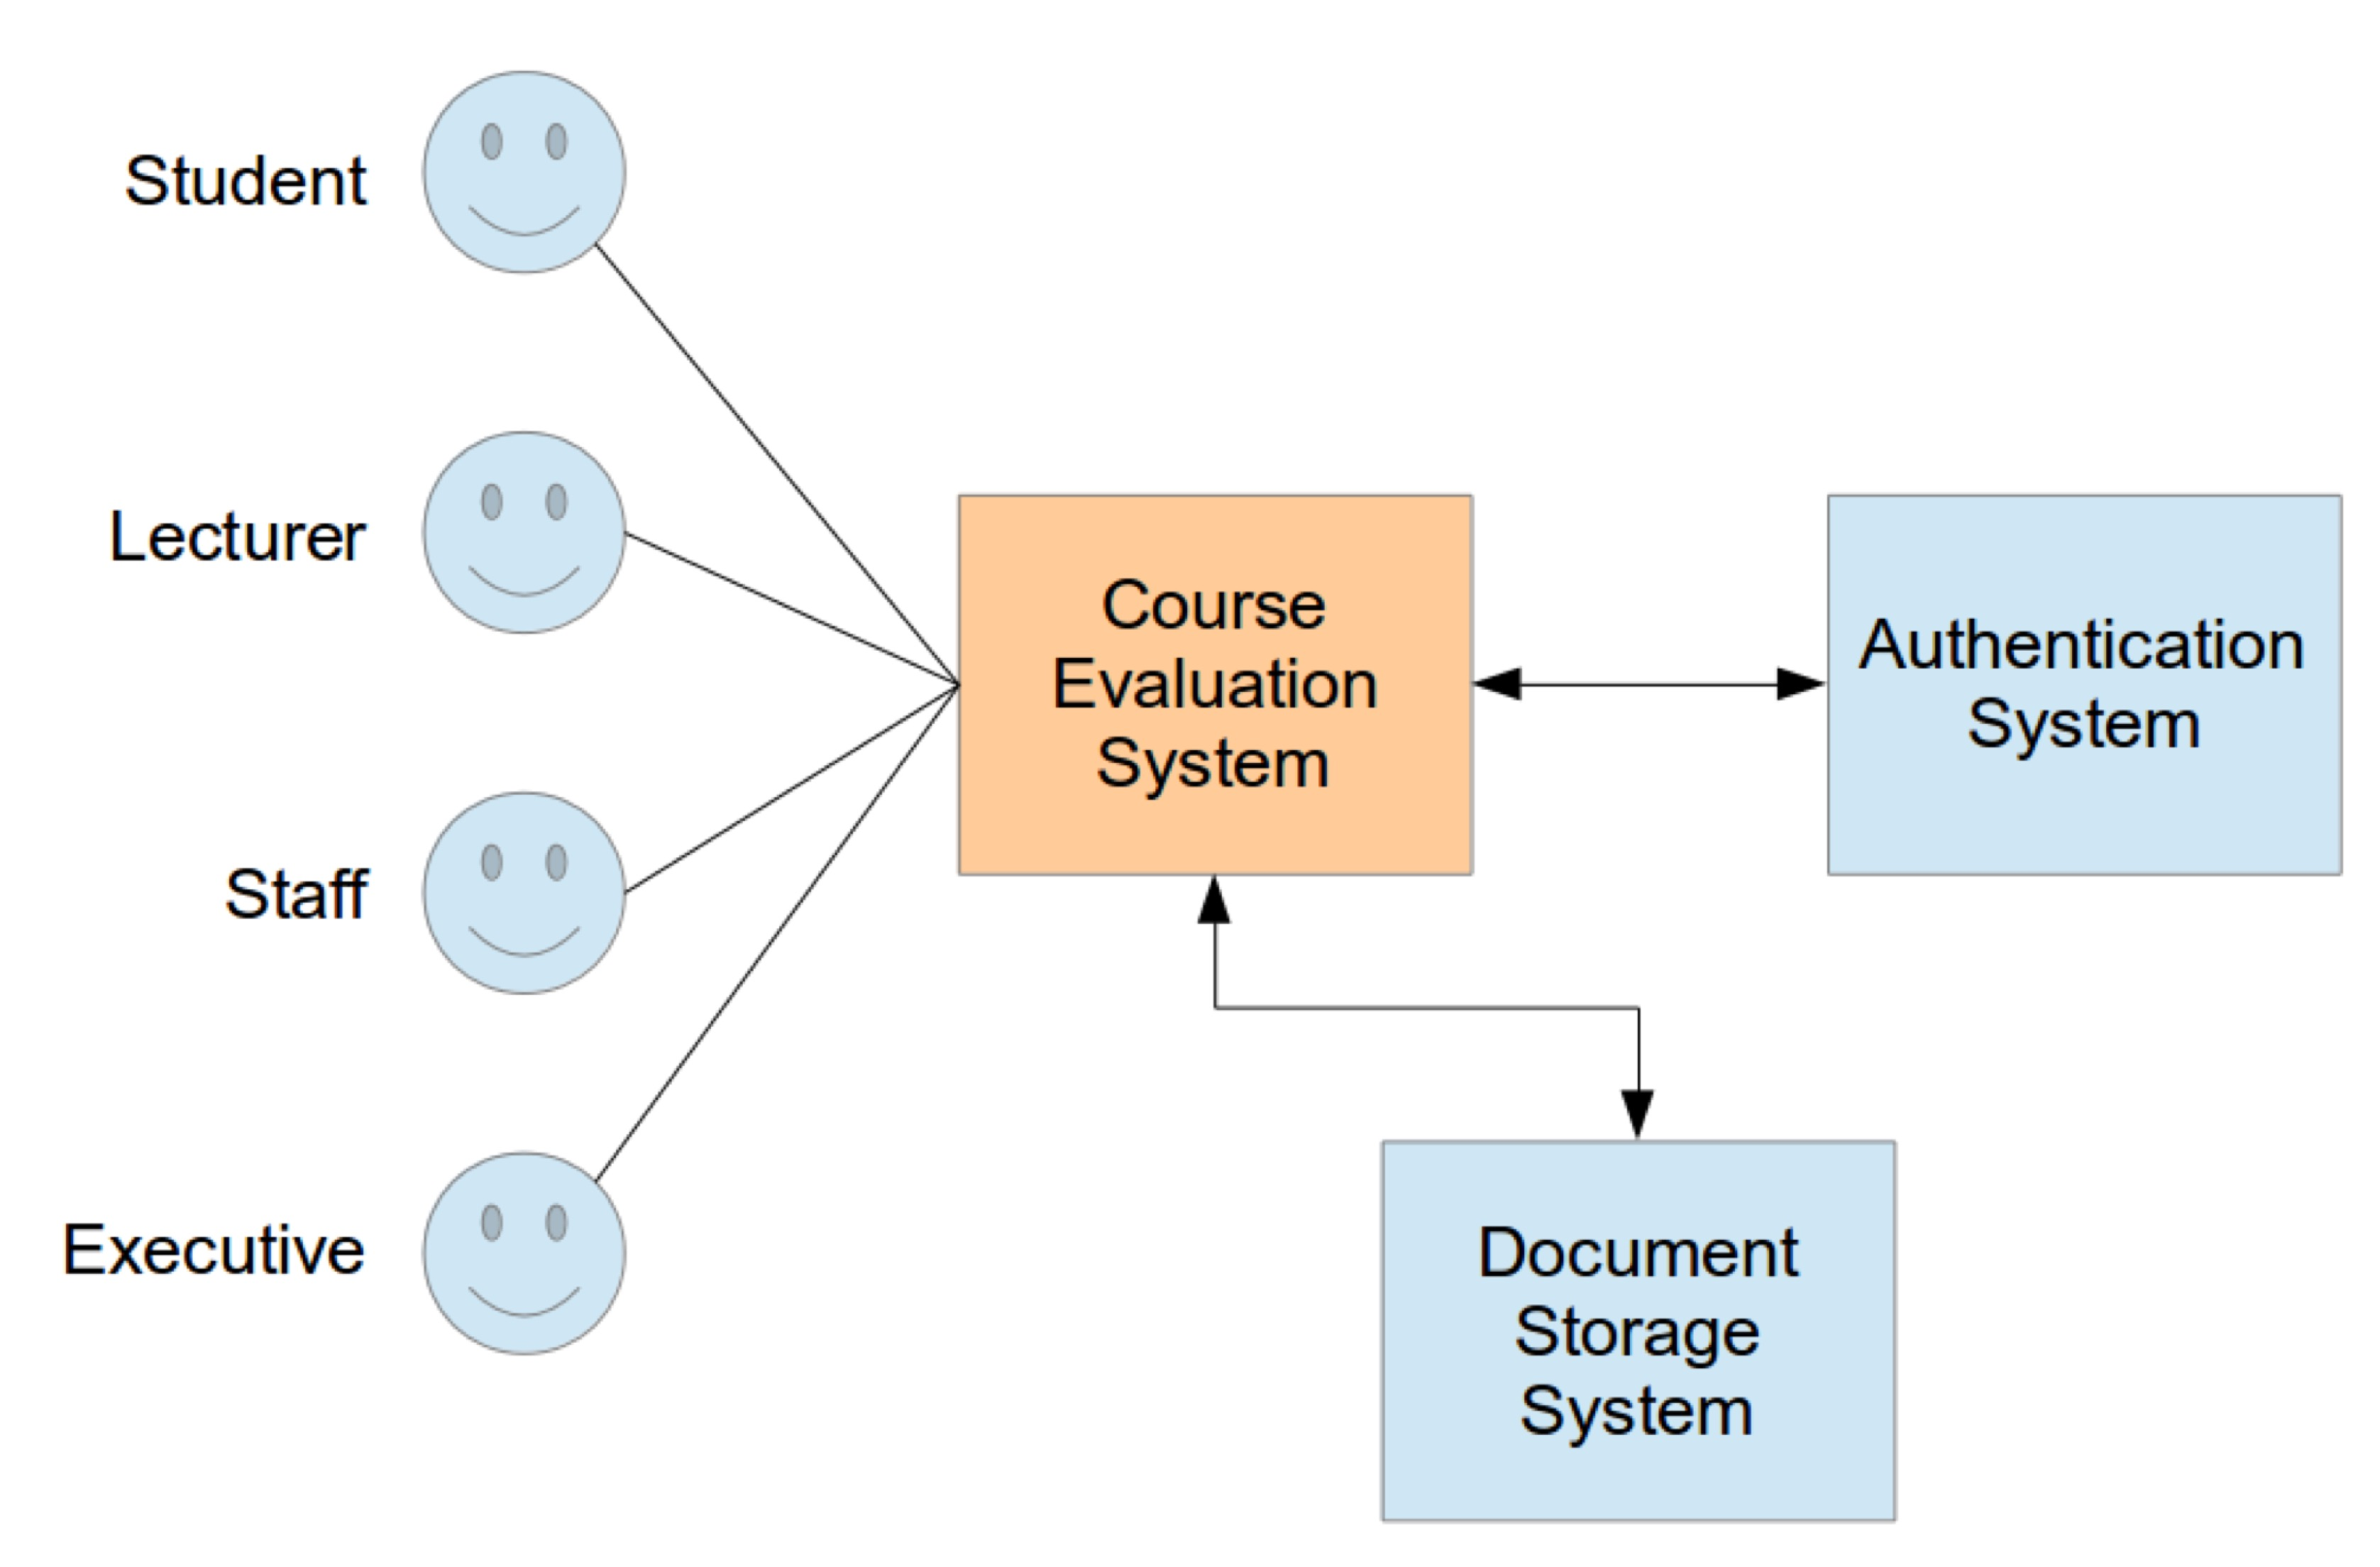
\includegraphics[keepaspectratio=true,width=10cm]{figure/f1}
\end{center}
\caption{System Perspective}
\label{fig2}
\end{figure}


The functions are summarised as:

\begin{itemize}
		\item Authentication: connects with the external SIIT Authentication system to check user logins and determine the access control
		\item Course Setup: allows staff to add new courses, including who is the lecturer/TA for each course
		\item Evaluation: allows students to perform the evaluation
		\item Reporting: allows different types of users to produce summary reports from a set of evaluations. PDF reports may be stored in the external SIIT Document Management system.
\end{itemize}




\subsection{Functions}

The functions of OCES are shown in Figure 2.

\begin{figure}[h]
\begin{center}
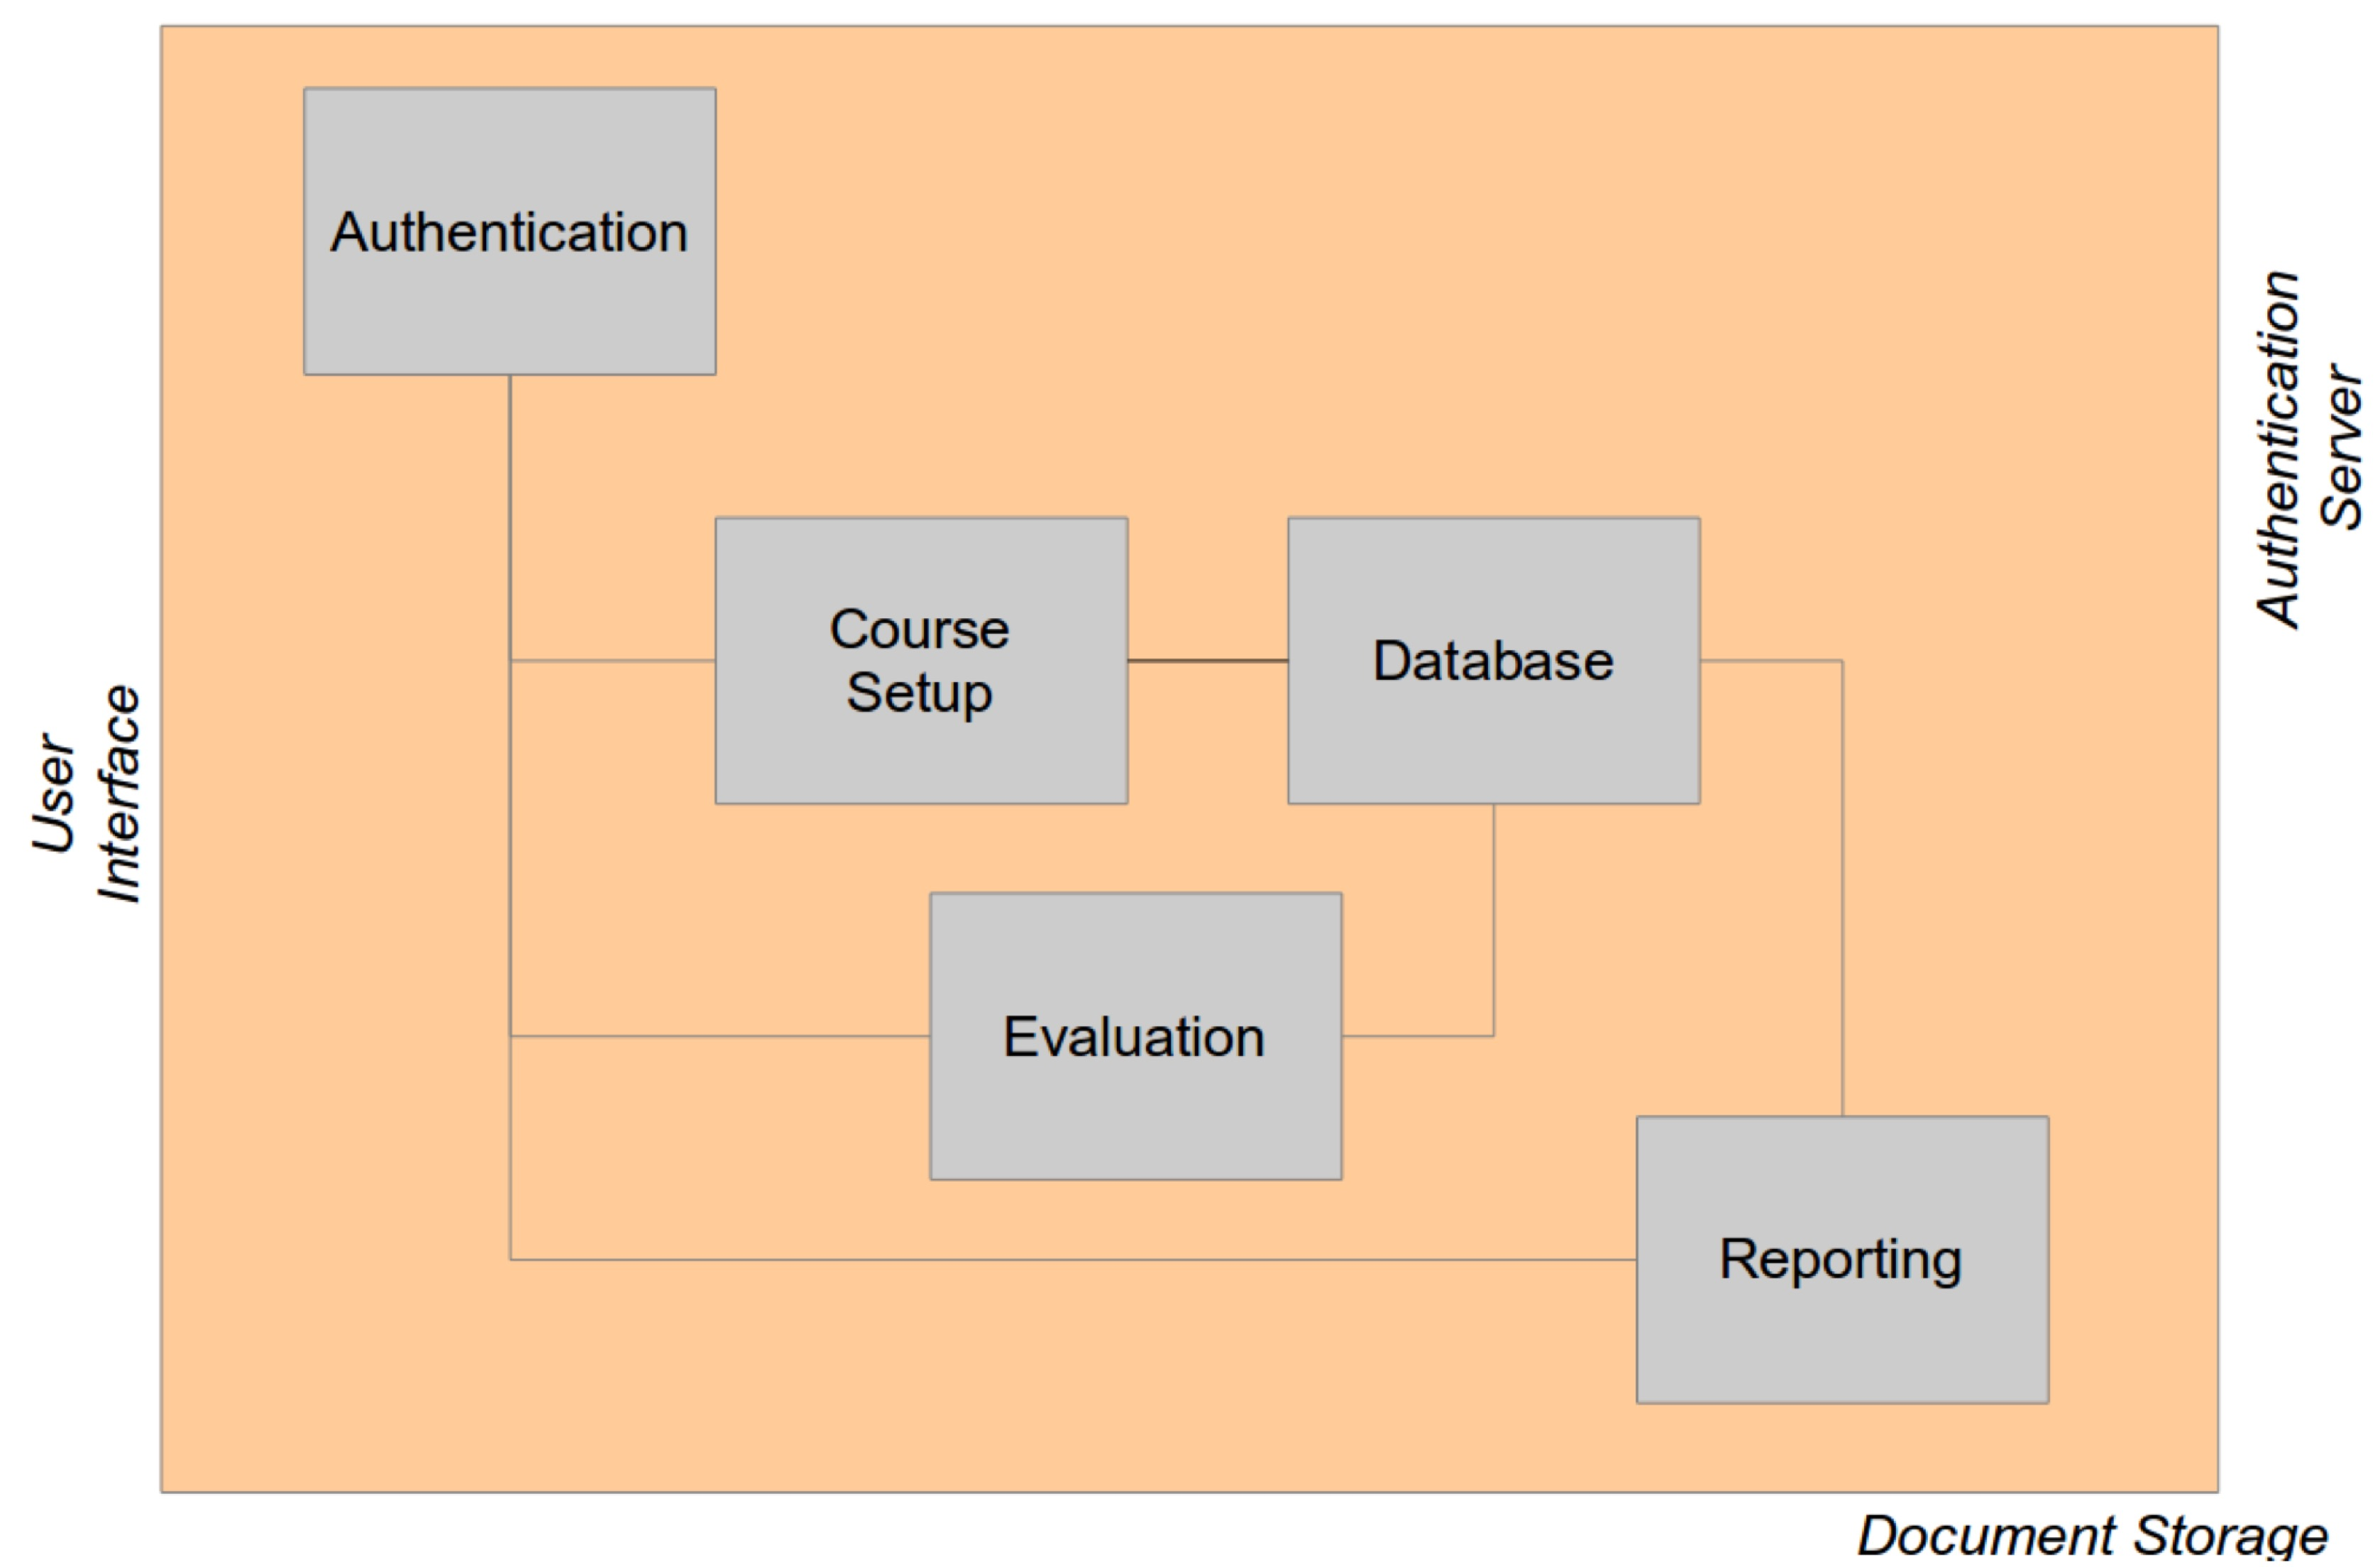
\includegraphics[keepaspectratio=true,width=10cm]{figure/f2}
\end{center}
\caption{System functions}
\label{fig1}
\end{figure}

\section{Requirements}

The requirements of the system are listed in the following subsections.


\subsection{General}

	\begin{itemize}
		\item[G1] OCES must ....
		\item[G2] OCES should ....
		\item[G3] OCES may ....
	\end{itemize}

\subsection{Authentication}

	\begin{itemize}
		\item[A1] The Authentication module must ....
		\item[A2] The Authentication module should ....
		\item[A3] The Authentication module may ....
	\end{itemize}

\subsection{Reporting}

	\begin{itemize}
		\item[R1] The Reporting module must  ....
		\item[R2] The Reporting module must  ....
		\item[R3] The Reporting module must  ....
	\end{itemize}

\chapter{Design Specification}
Describes how the features will work in your system. The design specification should include both 'what' and 'why'. That is, what is the design and why did you choose to design it that way. The 'why' part is also called rationale or justification, and is especially important when describing key parts of your system: “A key feature of our game is the manner in which points accrue when a player kills an opponent. Points are gained/lost according to the algorithm below ... . The reason we choose this approach is ... .”.


\section{System Architecture}
A high-level view of your system design. Similar to the ``System Description" section of the Requirements Specification, but in more detail and focusing on how the system works, not what it will do. You may include a block diagram showing the system components/modules and describe each briefly.


\section{Detailed Design}
A low-level view of your system design.

For each of the components identified in the System Architecture, give details of how they will be built. You may use different notation for the design, e.g. UML, block diagrams, pseudocode, message sequence charts, flow charts, hardware designs.



\chapter{System Manual}

Explanation of how the system was implemented and tested.


\section{Installation and Usage}


Assume students in next years senior project need to install your system on a new computer. The Installation section should list the steps to complete the installation. You do not need to give detailed steps of installing other peoples software (e.g. how to install MySQL server), only your own software/hardware. You should refer to specific files/directories in your electronic source code submission. For example:

\begin{enumerate}
	\item Install MySQL database server and Apache web server
	\item Import the database src/db/maindata.sql into MySQL
	\item Edit the file src/www/config.php to include appropriate database and password
	\item Copy all files from src/www/ into the web server base directory
	\item Access the website at http://example.com/courseeval/
	\item Login as ``admin" with password ``123456" and select a new password
\end{enumerate}

You should also explain important or non-obvious ways in using the system. Note that this is NOT a User Manual or help section: it does not have to cover all steps in using the system. For example, if you develop a website you do NOT need to explain the obvious features (such as login, search, sorting data, editing in forms). Instead explain only the non-obvious features. For example if you have a search feature on your website, and have included your own special query syntax, then explain that syntax.

If you have developed standalone software and/or hardware, you should explain how to start it. For example if your software is run on the command line, then give the syntax and main command line options for using it.

Do NOT include screen-shots (unless very useful in explaining non-obvious features).

\section{Implementation Overview}

A brief description of implementation-specific issues with your system. In other words, describe important aspects of the system that someone needs to understand the implementation, that are not already described in the Design Specification (do not repeat what is already in the Design Specification). You may start with a diagram or description that relates the architecture design with the source code that you developed. For example: ``The user login module is implemented in the file login.php, while the statistics processing module is in the set of files starting with stat\_."

An important part of this section is a list of the software/hardware components that you used, including versions. For example:

``Our website made use of the following software:

MySQL server version 5.5

Apache Web server version 2.4.1

Ubuntu Linux 14.04 LTS operating system"

This Implementation Overview is valuable for students in subsequent years that may need to view, understand and modify your code.

Do not include complete source code as that is submitted electronically. However you may refer to source code, either as a files or in source code snippets. In general, you want to put those snippets in the Appendices.

\section{Feature List}

In your Requirements Specification you identified what your system should do. Considering those requirements, you must summarise the 8 key features that you \textit{actually} deliver in your system and give the status of each feature: complete ($>$ 80\%), partial (40–80\%) or in the initial stages ($<$ 40\%) like in the following. It is up to you to decide how to divide your system/project into features. Choosing features that are too simple may result in penalties for the project. For some groups the feature list may be the same or similar to the components or requirements from the Requirements/Design Spec. For other groups they may be different.


\begin{enumerate}
	\item Combat System: Player can combat with either players or monsters.. (with physicals attack or magic attack) 

Feature status:   [ ]Complete\hspace*{1cm}     [ ]Partial\hspace*{1cm}    [ ]Initial


	\item Multi-player: Player can play the game with another players via the internet.
	
	
Feature status:   [ ]Complete\hspace*{1cm}     [ ]Partial\hspace*{1cm}    [ ]Initial

	\item Feature: short description of the feature
	
	
Feature status:   [ ]Complete\hspace*{1cm}     [ ]Partial\hspace*{1cm}    [ ]Initial

	\item .....
	

\end{enumerate}

\section{Test Results}
A description of how you tested your system, especially the completed features,  and what results were obtained. Consider the online course evaluation example. The website may be tested at different levels, including by potential users. Testing using fake data sets may be performed to check that the statistic calculations are correct. The data sets used should be described in the Test Results section. Testing by different users (students, admin, lecturer) may be performed to check that the features/workflow is as required. The number of users and how they tested should be described in the Test Results section.

Tests may be described informally (e.g. using text like “We asked 5 students to complete evaluations of 3 courses over a 1 week period. The feedback from the students was used to improve the website, in particular reducing the number of clicks needed to complete the evaluation from 5 down to 2.”) or formally (e.g. using tables of tests and results).

%%%% start of appendices %%%%
\appendix
\chapter{hello.java}
Do not put in this appendix complete source code as that is submitted electronically. However you may want to put some code snippets.  \LaTeX{} has a wonderful package called "listings" to include source code snipplets. See details in \cite{Wikipedi2016a}. An example is give below.

\lstinputlisting[language=Java]{./code/hello.java}


% Use IEEEtranS for bibilography that is sorted alphabetically. 
\bibliographystyle{IEEEtranS}
% Uncomment below to use IEEEtran so that the references are sorted by appearance.
%\bibliographystyle{IEEEtran}

\bibliography{seniorp}		


\end{document}